\documentclass[12pt]{article} 
\usepackage[utf8]{inputenc}

\title{Astronomy Notes}
\author{Aarush Gupta}
\date{2020}

\usepackage{natbib}
\usepackage{graphicx}
\usepackage{amsmath}
\usepackage{hyperref}
\usepackage[utf8]{inputenc}
\usepackage{fancyhdr}
\usepackage{color}
\usepackage{enumitem}
\usepackage{physics}

\renewcommand{\dd}{\mathrm{d}}

\pagestyle{fancy}
\fancyhf{}
\rhead{Aarush Gupta}
\lhead{Astronomy Notes}
\fancyfoot[C]{\thepage}

\urlstyle{same}

\begin{document}

\maketitle

\tableofcontents

\newpage

\section{Light and Continous Spectra}

\subsection{Parallax}

\textbf{Distance Parallax}: Calculating distance based on angle between two seperate observations.
\begin{align*}
    d = \frac{1\;\text{AU}}{\tan{p}}
\end{align*}
This can also be written as
\begin{align*}
    d = \frac{1}{p''}
\end{align*}
if $d$ is measured in parsecs.

Small $p$ $\to$ huge error in $d$, so error-prone for objects very far away.

\subsection{Magnitude}

One magnitude corresponds to a $\sqrt[5]{100} \approx 2.512$ facto difference in brightness, created by Hippoarchus. Observable magnitudes range from Sun (-26.83) to +30 for faintest galaxies. This leads to:
\begin{align*}
    F_2/F_1 = 100^{(m_1 - m_2)/5} \\
    m_1 - m_2 = -2.5\log{\left(\frac{F_2}{F_1}\right)}
\end{align*}
Noting that $F = \frac{L}{4\pi r^2}$:
\begin{align*}
    d = 10^{(m - M + 5)/5}\;\text{pc} \\
    m - M = 5\log{\left(\frac{d}{10\;\text{pc}}\right)}
\end{align*} 

\subsection{Wave Nature of Light}
Diffraction experiments revealed that light was a wave, where $\lambda\nu = c$ and $c = \frac{1}{\sqrt{\mu_0\varepsilon_0}}$.

\begin{center}
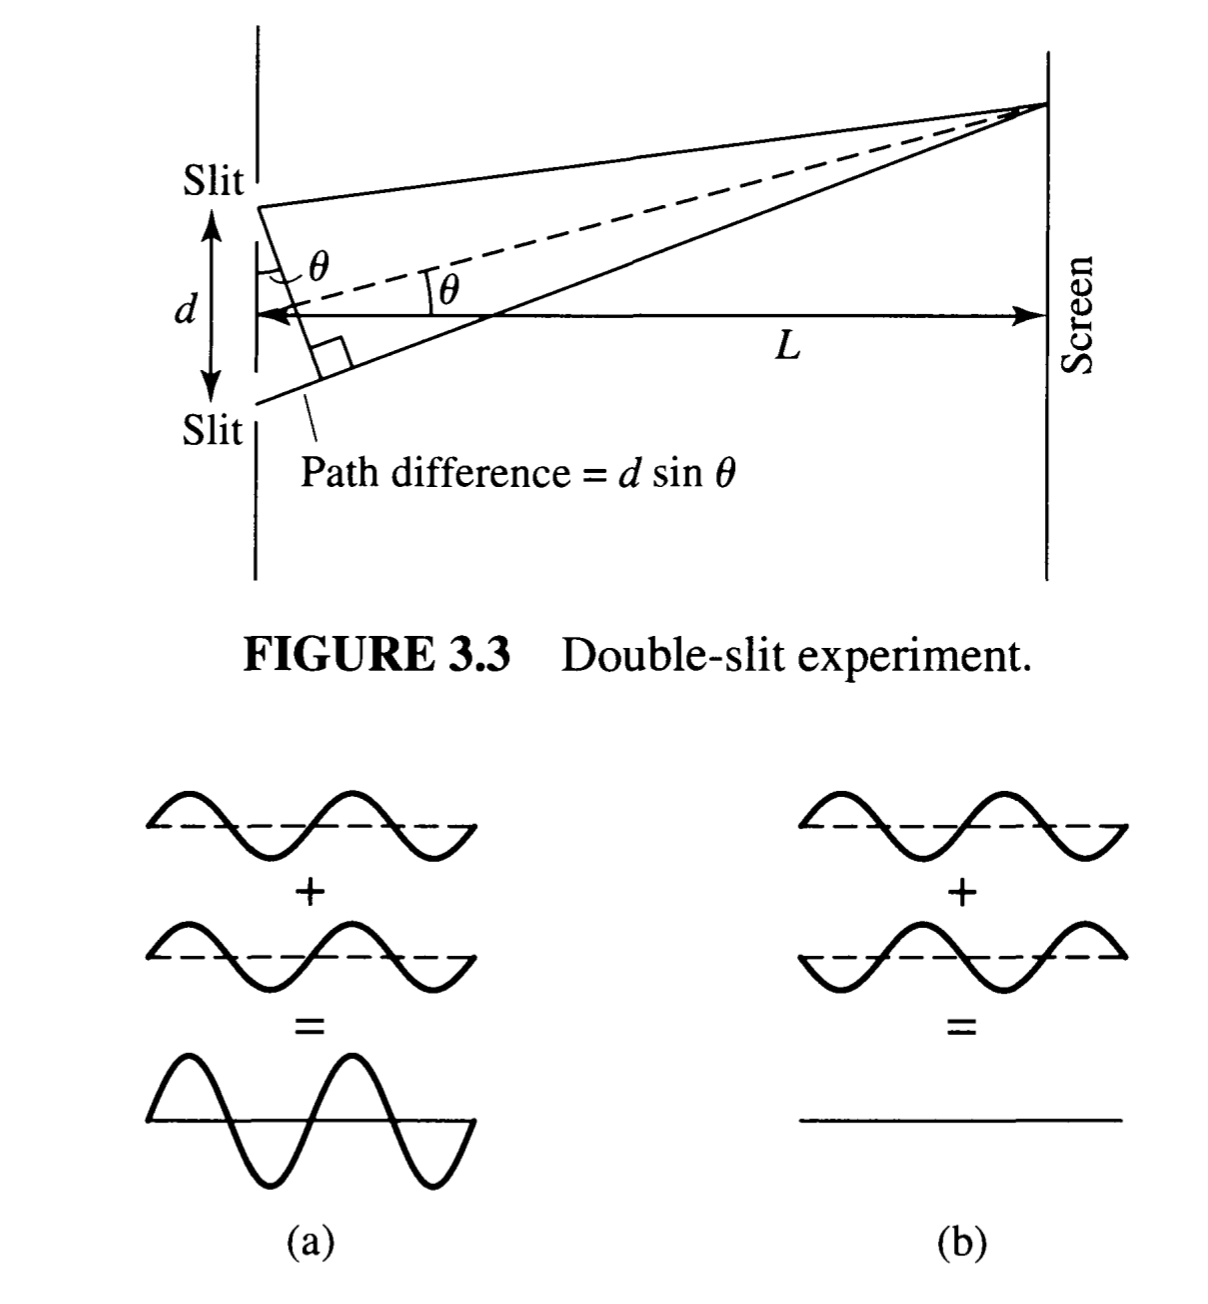
\includegraphics[scale=0.3]{Figures/DoubleSlitDiagram}
\end{center}

For double-slit diffraction, the path length difference is around $d\sin\theta$, so:
\begin{align*}
    d\sin\theta = \begin{cases} 
        n\lambda & \text{Constructive interference (bright fringes)} \\
        \left(n-\frac{1}{2}\right)\lambda & \text{Destructive interference (dark fringes)}
     \end{cases}
\end{align*}
where $n$ is an integer for the \textbf{order} of the minima/maxima.

Maxwell's theory of EM described light as an EM wave, with changing E and B fields inducing each other. Note that amplitudes of fields $E_0/B_0 = c$. The rate of energy transmission is given by \textbf{Pontying Vector}:
\begin{align*}
    \textbf{S} = \frac{1}{\mu_0}\textbf{E}\times\textbf{B} \\
    \left<S\right> = \frac{1}{2\mu_0}E_0B_0
\end{align*}

Because of its momentum, light exerts radiation pressure.

\begin{align*}
    P = \frac{\left<S\right>}{c}\cos\theta\;\text{ (absorption)} \\
    P = \frac{2\left<S\right>}{c}\cos^2\theta\;\text{ (reflection)}
\end{align*}

\subsection{Thermo and Stellar Spectra}

Below are Stefan-Boltzmann and Wien's Laws, respectively:
\begin{align*}
    L = \varepsilon\sigma AT_e^4\\
    \lambda_{max}T = b
\end{align*}

Stefan-Boltzmann Law uses the "effective temperature" of a star. It can also be used to find the surface flux:
\begin{align*}
    F_{surf} = L/4\pi R^2 = \sigma T_e^4
\end{align*}

Derived from the \textbf{Planck Function}: $B_{\nu}(T)\;d\nu$ and $B_{\lambda}(T)\;d\lambda$ represent the radiant energy per unit time per unit area per unit solid angle.

\begin{align*}
    B_{\lambda}(T) = \frac{2hc^2/\lambda^5}{e^{hc/\lambda kT} - 1} \\
    B_{\nu}(T) = \frac{2h\nu^3/c^2}{e^{h\nu/kT} - 1}
\end{align*}

Indeed,
\begin{align*}
    \int_{0}^{\infty}B_{\lambda}(T)\;d\lambda = \frac{\sigma T^4}{\pi}
\end{align*}

Before Planck's Law, two approximations were present:
\begin{align*}
    B_{\lambda}(T) = \begin{cases}
        \frac{2ckT}{\lambda^4} & \lambda\to\infty \\
        a\lambda^{-5}e^{-b/\lambda T} & \lambda\to 0
    \end{cases}
\end{align*}

The first approximation is called \textbf{Rayleigh-Jean's Law}, failed due to \textbf{ultraviolet catastrophe}, which meant that $B(T)\to\infty$ as $\lambda\to 0$.
The second one is \textbf{Wien's Approximation}, which is just empirical.


\subsection{Color}
Although \textbf{bolometric magnitudes} (magnitudes measured over all wavelengths) are used in calculations, detectors usually use a certain part of the spectrum. This information can be contained in the sensitivity function $S(\lambda)$, the fraction of flux detected at a certain wavelength. Then, flux at a certain wavelength is $F(\lambda)S(\lambda)\;d\lambda$

Magnitudes can be assigned for ultraviolet, blue, and visual. Then, we can also define color indices, like so:
\begin{align*}
    U - B = M_U - M_B \\
    B - V = M_B - M_V
\end{align*}

$U$, $B$, and $V$ are apparent color magnitudes. Distance plays no role in these color indices, just the actual absolute color magnitudes. Lower U-B and B-V indices correspond to more ultraviolet and blue stars respectively, and vice versa (since higher absolute magnitude means less flux).
A bolometric correction can also be defined as so:
\begin{align*}
    BC = m_{bol} - V = M_{bol} - M_V
\end{align*}
To try to make $BC$ always negative, $C_{bol}$ introduced:
\begin{align*}
    m_{bol} = -2.5\log{\int_{0}^{\infty}F_{\lambda}\;d\lambda} + C_{bol}
\end{align*}
It didn't work though because some supergiants have positive BCs.

Then,
\begin{align*}
    U-B = -2.5\log{\frac{\int F_{\lambda}S_U(\lambda)}{\int F_{\lambda}S_B(\lambda)}} + C_{U-B}\\
    B-V = -2.5\log{\frac{\int F_{\lambda}S_B(\lambda)}{\int F_{\lambda}S_V(\lambda)}} + C_{B-V}
\end{align*}

Note that $\left(\frac{R}{r}\right)^2$ factor cancels out in the fraction, meaning no dependence on distance. An approximation can also be used when only a certain region of light can be observed at full intensity, and the rest is zero. The range of observable wavelengths is the \textbf{bandwidth}, $\Delta\lambda$.

\begin{align*}
    U-B = -2.5\log{\left(\frac{B_{\lambda, U}\Delta\lambda_U}{B_{\lambda, B}\Delta\lambda_B}\right)} + C_{U-B} \\
    B-V = -2.5\log{\left(\frac{B_{\lambda, B}\Delta\lambda_B}{B_{\lambda, V}\Delta\lambda_V}\right)} + C_{B-V}
\end{align*}

A graph of U-B vs. B-V is called a color-color diagram. Ideal blackbodies would lie along a straight line, and hotter stars tend to lie closer to this line.

\begin{center}
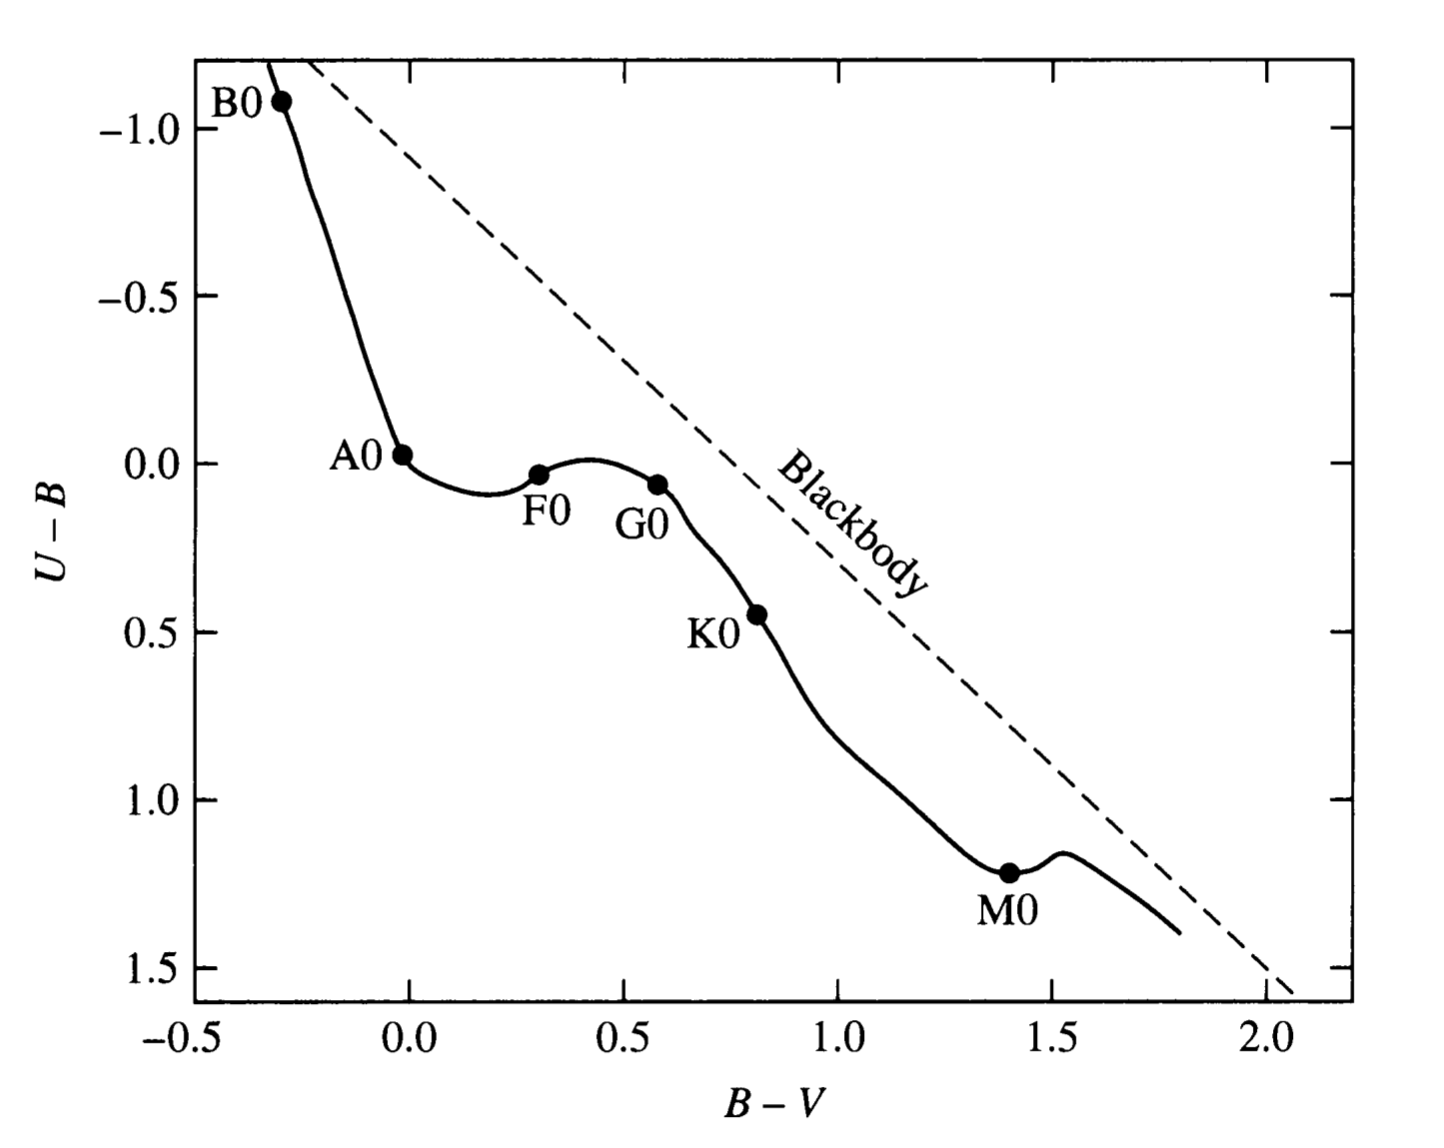
\includegraphics[scale=0.5]{Figures/ColorColorDiagram}
\end{center}

\section{Spectral Lines}

\subsection{Measuring Spectral Lines}

Measuring the lengths of spectral lines can be done using diffraction grating and interference. Maxima would occur at $$d\sin\theta = n\lambda$$ and max resolving power is $$\Delta\lambda = \frac{\lambda}{nN}$$ where $N$ is number of grating lines illuminated.

\begin{center}
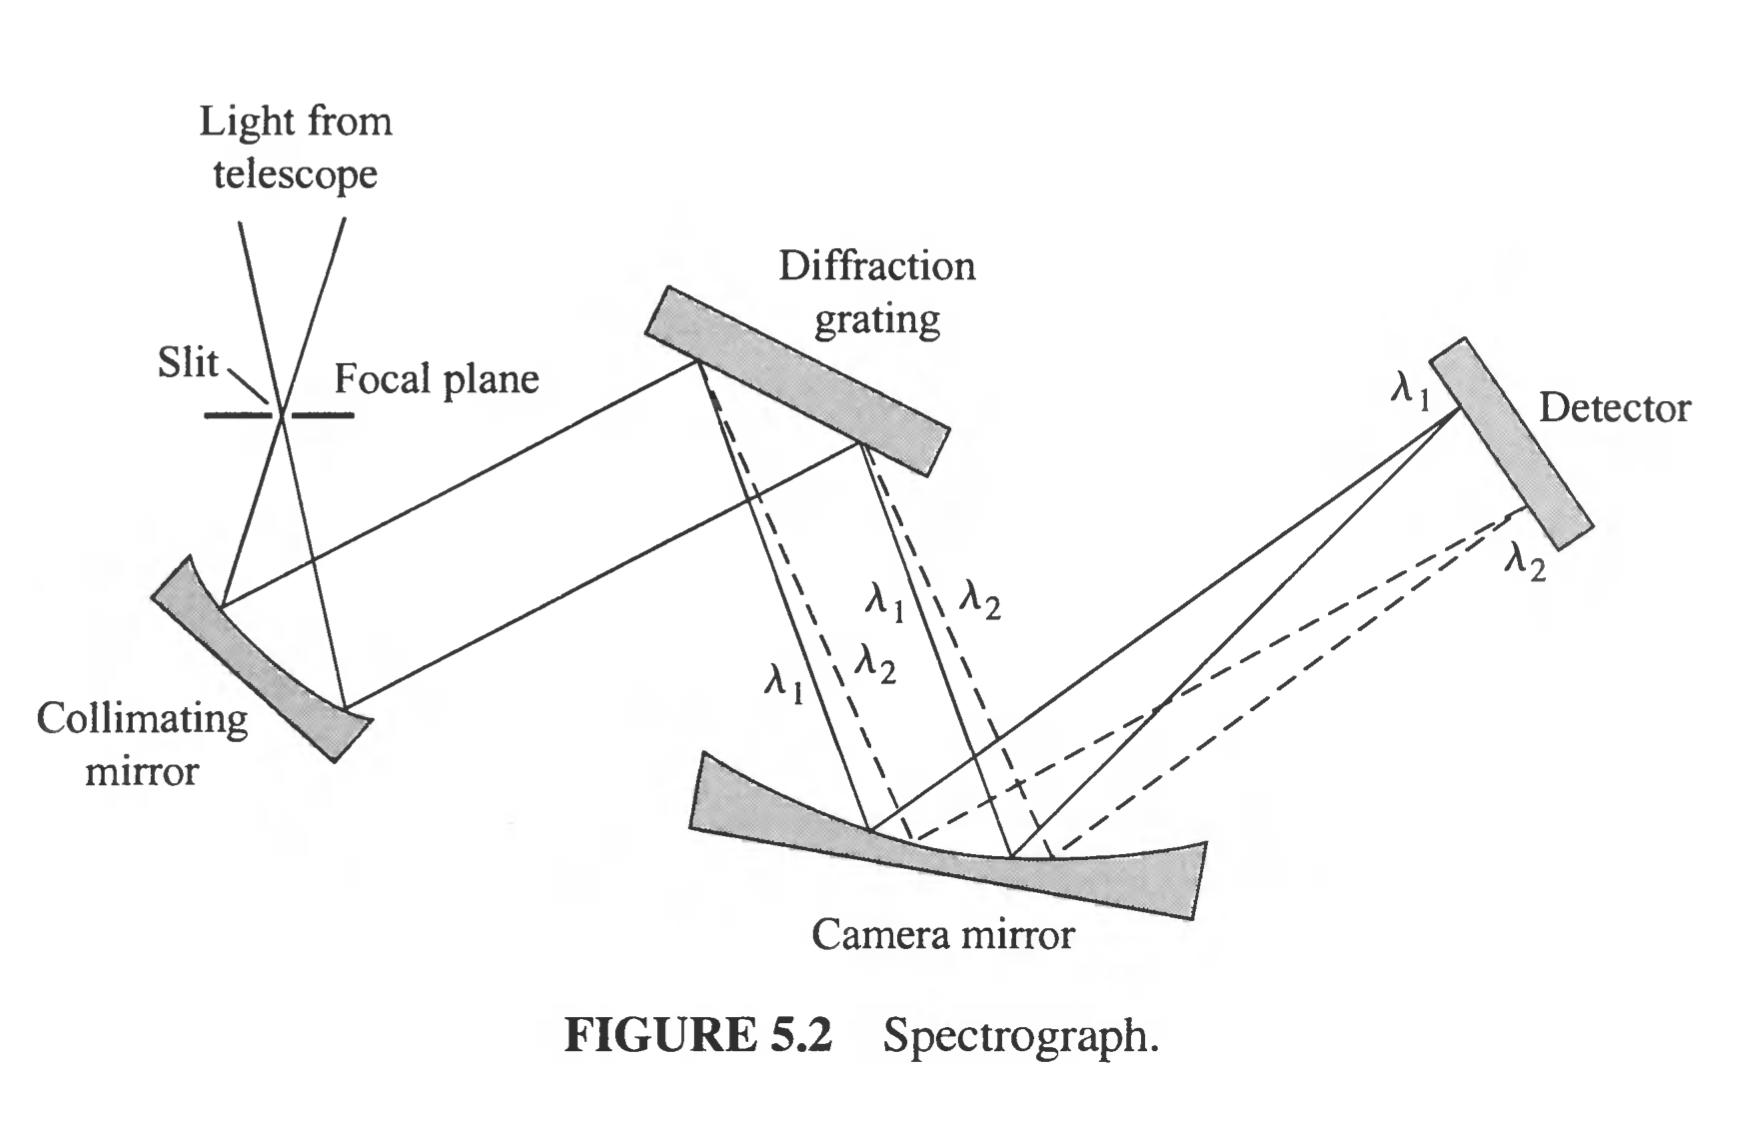
\includegraphics[scale=0.5]{Figures/Spectrograph}
\end{center}

\subsection{Derivation of Hydrogen Lines, Bohr Model}

Quantum mechanics provided explanation for spectral lines discovered by Joseph van Fraunhofer (\textbf{Fraunhofer lines}) and others.

Balmer discovered the following empirical formula for the \textbf{Balmer lines}, transitions from n=2 orbital of hydrogen, and further generalized it to
\begin{align*}
    \frac{1}{\lambda} = R_H\left(\frac{1}{m^2} - \frac{1}{n^2}\right)
\end{align*}

However, Bohr model of atom and angular momentum quantization helped explain this. Using these conditions and equations, where $\mu$ is reduced mass:
\begin{align*}
    F_e = \frac{1}{4\pi\epsilon_0}\frac{q_1q_2}{r^2} \\
    L_n = n\hbar = \mu vr \\
    F_c = \frac{\mu v^2}{r}
\end{align*}

the radii of orbit can be shown to be quantized by Bohr's radius, $a_0$
\begin{align*}
    r_n = \frac{4\pi\epsilon_0\hbar^2}{\mu e^2}n^2 = a_0n^2
\end{align*}

Using the Virial theorem, $$E_n = -\frac{1}{8\pi\epsilon_0}\frac{e^2}{r_n}$$.

Then, note that $$ \frac{hc}{\lambda} = E_{\nu} = E_n - E_m $$

Substituting the expression for $r_n$ and simplifying, $$R_H = \frac{\mu e^4}{64\pi^3\epsilon_0^2\hbar^3c}$$

\textbf{Selection rules} play a factor in what transitions are even possible, however.

Despite the quantization of photon frequencies from emission and absorption, things like magnetic fields may cause slight differences due to their effects on energy levels; this \textbf{Zeeman Effect} is quantified like so: $$\nu = \nu_0 \pm \frac{eB}{4\pi\mu}$$

\subsection{Kirchoff's Laws}

\begin{enumerate}
    \item Hot, dense gas or hot solid $\to$ continuous emission spectrum (Planck Blackbody)
    \item A hot, diffuse gas $\to$ emission lines, downward electron transitions
    \item Cool, diffuse gas $\to$ absorption lines from continuous spectrum behind it
\end{enumerate}

\subsection{Spectral Line Profiles}

\textbf{Equivalent Width:} $\int \dfrac{F_c - F_\lambda}{F_c}\;\dd\lambda$ (accounts for both depth and width of curve)
\begin{itemize}
    \item Sometimes used to calculate density of atoms of a certain element using a \textbf{curve of growth}
\end{itemize}

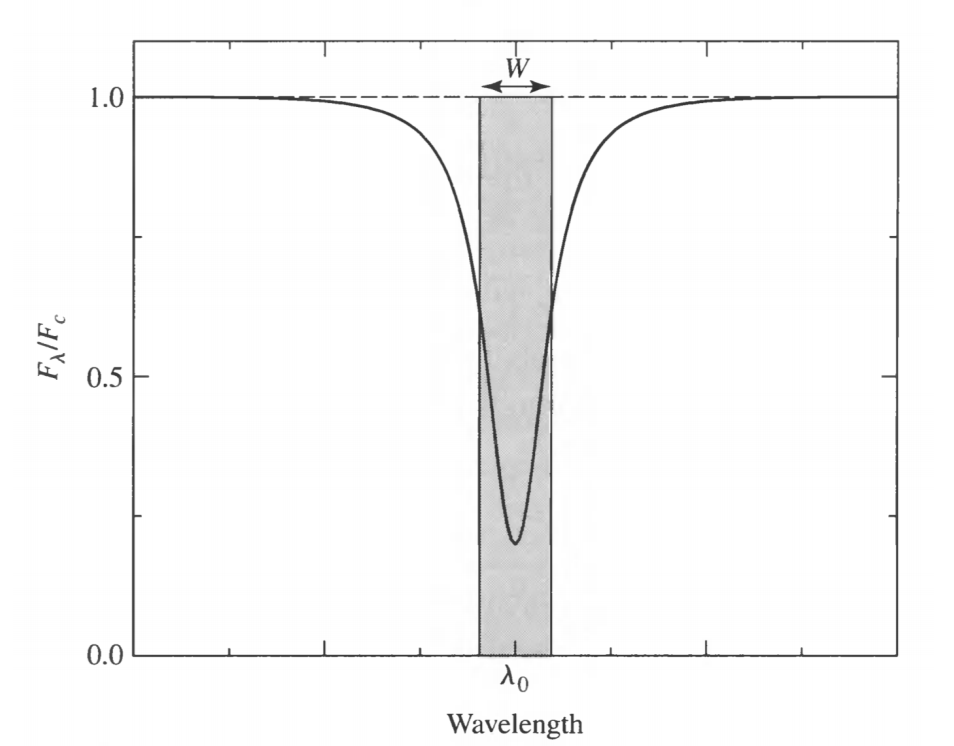
\includegraphics[scale=0.5]{Figures/EquivalentWidth.png}

There are several reasons why spectral lines are broadened (i.e. not perfectly thin)
\begin{itemize}
    \item \textbf{Damping/Lorentz Profile:}
    \begin{itemize}
    \item \textbf{Natural Broadening:} Uncertainty in energy ($\Delta E\Delta t \approx\hbar$) and $E = hc/\lambda$ $\implies$ $\Delta\lambda = \dfrac{\lambda^2}{2\pi c}\left(\frac{1}{\Delta t_i} + \frac{1}{\Delta t_f}\right)$
    \item \textbf{Pressure/Collisional Broadening:} Electric fields of neighboring atoms lead to shift in energy levels $\implies$ $\Delta\lambda = \frac{\lambda^2}{\pi c\Delta t_0} = \frac{\lambda^2v}{\pi c\ell} = \frac{\lambda^2n\sigma}{\pi c}\sqrt{\frac{2kT}{m}}$ (less broadening for low density stars like supergiants)
    \end{itemize}
    \item \textbf{Doppler Broadening:} Random motions of atoms lead to Doppler shift uncertainty: $v_p = \sqrt{2kT/m}$ and $\Delta\lambda/\lambda \approx \frac{2v}{c} \implies \Delta\lambda = \frac{2\lambda}{c}\sqrt{\frac{2kT}{m}}$
\end{itemize}

The \textbf{Voigt profile} is a combination of both the damping and doppler profiles, as shown below:

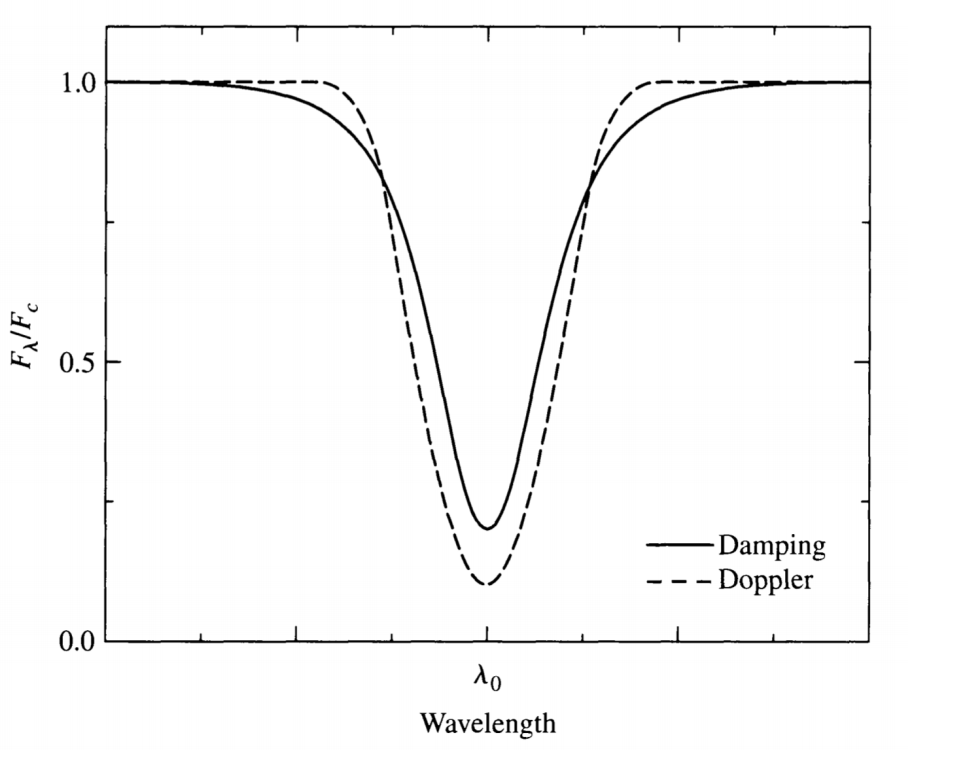
\includegraphics[scale=0.5]{Figures/VoigtProfile.png}

\section{Classifying Stellar Spectra}
Spectral types from early to late (can be further divided into 0-9): \textbf{O, B, A, F, G, K, M, -- L, T} (later of which are \textbf{brown dwarfs}. Many stellar spectra classified by Annie Jump Cannon, put into Henry-Draper Catalogue.

Morgan-Keenan luminosity classes are also used to describe stars:
\begin{itemize}
    \item \textbf{Ia-O:} Extreme, luminous supergiants
    \item \textbf{Ia:} Luminous supergiants
    \item \textbf{Ib:} Less luminous supergiants
    \item \textbf{II:} Bright giants
    \item \textbf{III:} Normal giants
    \item \textbf{IV:} Subgiants
    \item \textbf{V:} Main sequence (dwarf) stars
    \item \textbf{VI, sd:} Subdwarfs
    \item \textbf{D:} White dwarfs
\end{itemize}

Listed below are characteristics for stellar spectra of different types and a graph to illustrate them:\newline
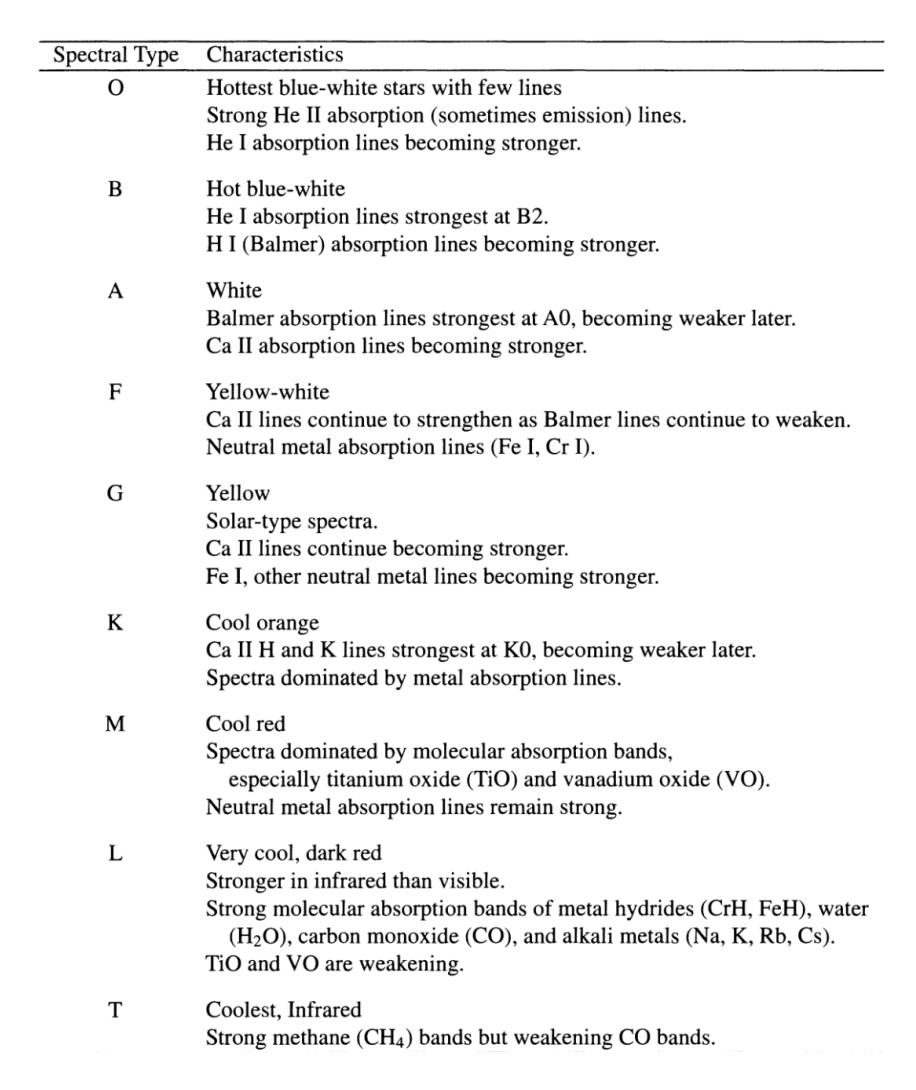
\includegraphics[scale=0.6]{Figures/SpectraClassification.png}
\newline
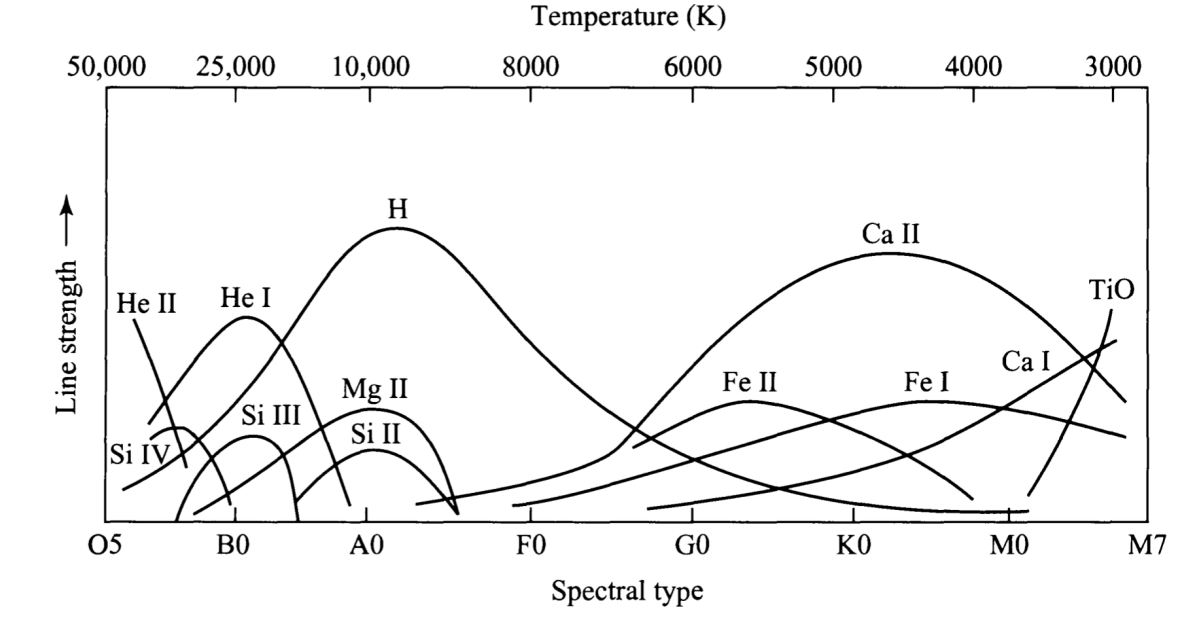
\includegraphics[scale=0.5]{Figures/LineStrengthChart.png}



\textbf{Boltzmann Equation:} (Ratio of electrons in different energy levels)

$$\dfrac{N_b}{N_a} = \dfrac{g_b}{g_a}e^{-(E_b - E_a)/kT}$$ where $g$ is number of degenerate states)

\textbf{Saha Equation:} (Ratio of ionized to normal atoms)

$$\dfrac{N_{i+1}}{N_i} = \dfrac{2Z_{i+1}}{n_eZ_i}\left(\frac{2\pi m_ekT}{h^2}\right)^{3/2} = \dfrac{2kTZ_{i+1}}{P_eZ_i}\left(\frac{2\pi m_ekT}{h^2}\right)^{3/2}$$ (Conversion based on $P_e = n_ekT$)\newline\newline

These two equations can be used to determine the fraction of atoms that are available to form a certain type of spectral line, since the strength of spectral lines form depends on both the fraction of ionization as well as the probability of the energy states of the atom.

This explains why Balmer lines cannot be formed at arbitrarily high temperatures, since a majority of hydrogen atoms would actually be ionized then (the \textbf{partial ionization zone} occurs at around 10,000 K). Instead, the curve looks like this based on the equations:

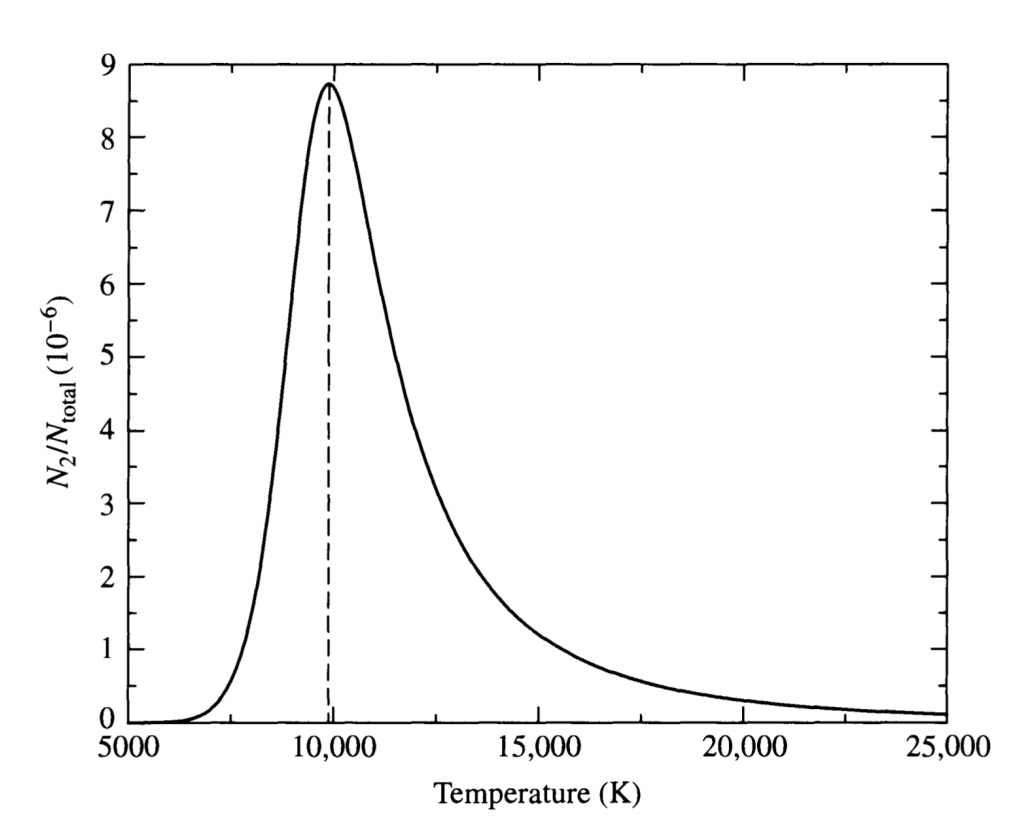
\includegraphics[scale=0.5]{Figures/BalmerLineCurve.png}

Additionally, formation of spectral lines depends not only on the amount of a certain element, but what fraction of it is actually able to form lines (e.g. there are more calcium than hydrogen lines formed by the Sun even though there is obviously more hydrogen)

\subsection{Hertzprung-Russell Diagram}
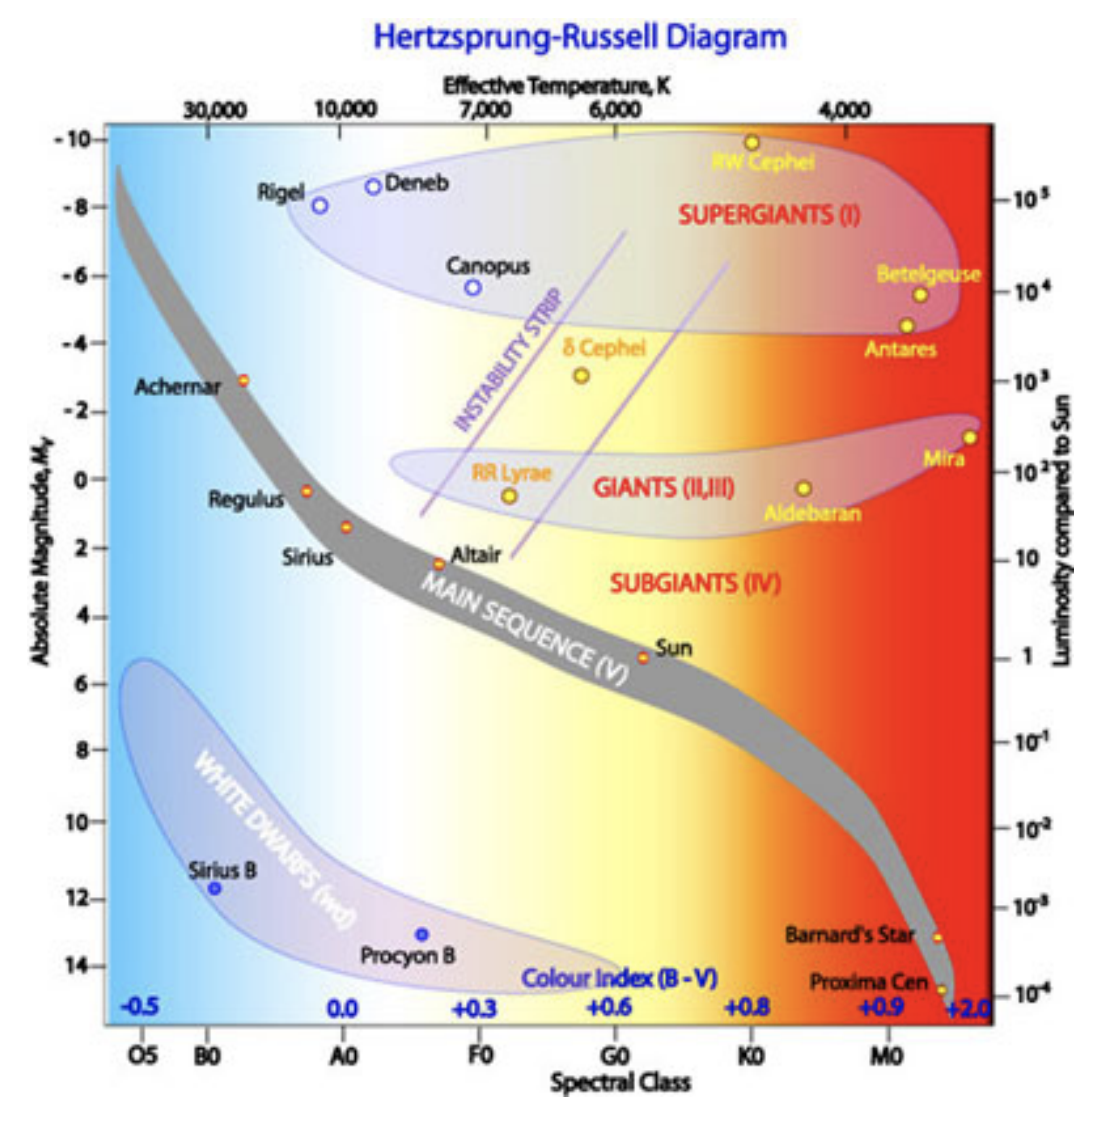
\includegraphics[scale=0.5]{Figures/HRDiagram.png}

\begin{itemize}
\item Bigger stars towards the top right, since higher luminosity, lower temperature lead to increased radius based on Stefan-Boltzmann Law: $R = \frac{1}{T_e^2}\sqrt{\frac{L}{4\pi\sigma}}$. \textit{Lines of constant radius are diagonal with a negative slope on the diagram.}
\item A star's mass is the determining factor for where it lies on the main sequence (early type stars are massive, vice versa) 
\item There a clear mass-luminosity relation for the main sequence. The slight width of \textbf{main sequence} (80-90\% of stars) is due to slight differences and evolution in stars along it.
\item Special groups include \textbf{white dwarfs, dwarfs, giants, and supergiants}.
\end{itemize}

\section{Observational Astronomy and Telescopes}

\subsection{Reflection and Refraction}
\textbf{Snell's Laws:}
\begin{itemize}
    \item Reflection: $\theta_1 = \theta_2$\newline
    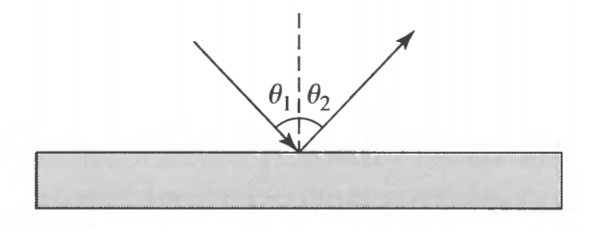
\includegraphics[scale=0.5]{Figures/Reflection.png}
    \item Refraction: $n_1\sin\theta_1 = n_2\sin\theta$\newline
    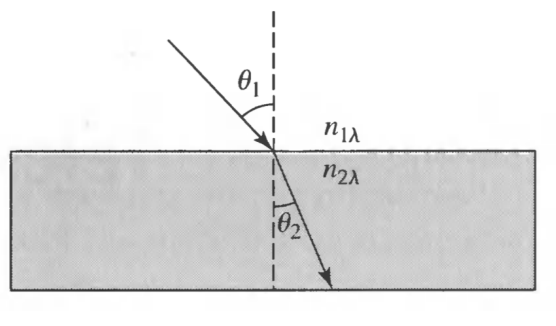
\includegraphics[scale=0.5]{Figures/Refraction.png}

    \item Lensmaker Formula (note the diagram which illustrates sign convention): $$ \frac{1}{f_{\lambda}} = (n_{\lambda} - 1)\left(\frac{1}{R_1} + \frac{1}{R_2}\right) $$
    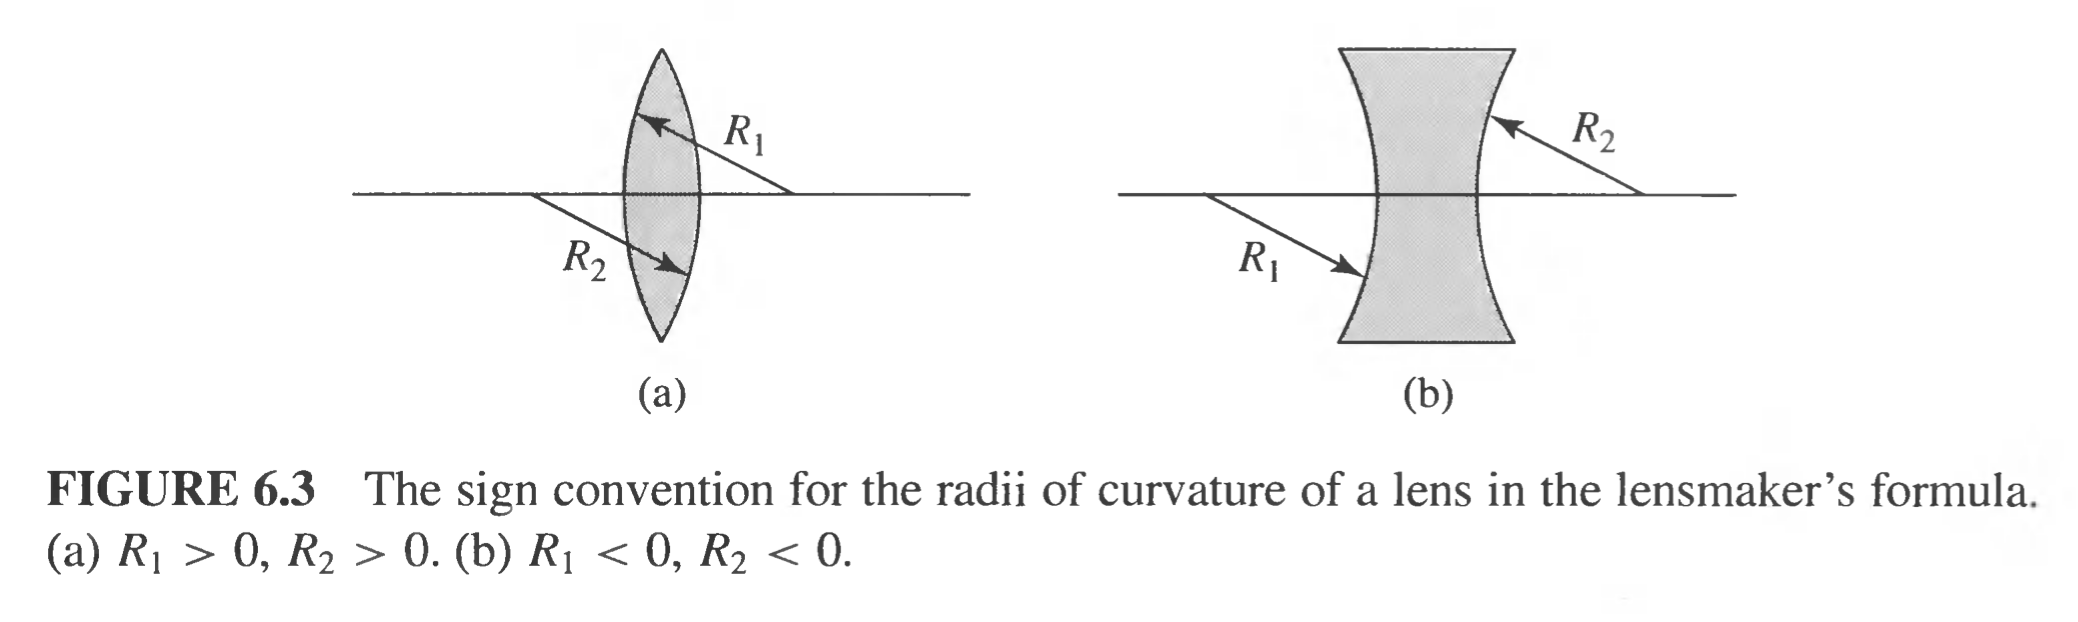
\includegraphics[scale=0.4]{Figures/LensmakerSignConvention.png}
    \item \textbf{Focal length is wavelength independent} (for spherical mirrors $f = R/2$)

\end{itemize}
\subsection{Resolution}

    $$ y = f\tan\theta \approx f\theta\;\; (\theta \ll 1) \implies \dv{ \theta}{y} = \frac{1}{f}$$
    Angular resolution (linear seperation of angular distances) increases as focal length increases (\textbf{plate scale}).

    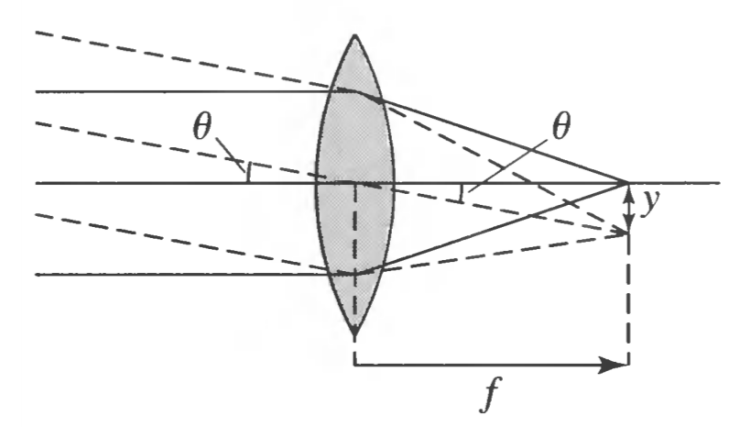
\includegraphics[scale=0.7]{Figures/PlateScale.png}

    General form of destructive interference: $\sin\theta = m\frac{\lambda}{D}$, where $D$ is the width of the slit.

    For a point source, the first-order minimum is at $m = 1.22$. Thus, the Rayleigh criterion states that the maximum angular resolution is $$\sin\theta = 1.22\frac{\lambda}{D} \implies \boxed{\theta \approx 1.22\frac{\lambda}{D}}$$

    Earth's turbulent atmosphere also plays a role in image resolution/quality, and for a certain location and time this is defined as the \textbf{seeing}.

\subsection{Aberration}
\begin{itemize}
    \item \textbf{Chromatic Aberration}: Since focal lengths may be wavelength-dependent for lenses, different colors can have different focal points which leads to a blurred out image (effect can be diminished using \textit{correcting lenses})
    \item \textbf{Spherical Aberration:} Imperfections in the lens's surface can lead to light not being focused at a single focal point (instead, parabaloids can be used to reduce this effect)
    \item \textbf{Coma:} If the source is not exactly on the optical axis, elongated images can be produced (focal length depends on angle of incoming light)
    \item \textbf{Astigmatism:} Light converges at slightly different locations on the focal plane
    \item \textbf{Curvature of Field:} Image converges on a curved surface
    \item \textbf{Distortion of Field:} Plate scale depends on distance from optical axis
    
    Aperture size does \textbf{not} affect brightness. However, the illumination (light power per unit area) $J$ follows the following relation: $$J \propto \frac{A_o}{A_i} \propto \frac{D^2}{f^2}$$. Then, $F = \frac{f}{D}$ is defined as focal ratio, and can be written in the format "f/{F}".
\end{itemize}

\subsection{Telescopes}

\textbf{Objective lenses} collect as much light as possible, while \textbf{eyepieces} allow the image to be viewed. In fact, the magnification of an image is $$m = \frac{f_{\text{obj}}}{f_{\text{eye}}}$$

However, objective lenses cannot be made too large since this would decrease the illumination significantly which would not allow the image to even be seen.

\subsubsection{Reflecting Telescopes}

Replacing the objective lens with a mirror can solve many issues:
\begin{itemize}
    \item Only one surface needs to be ground to precision (rather than an entire lens)
    \item Less weight, a "honeycomb structure" can be used to support the mirror
    \item \textbf{Active/adaptive optics} and pressure pads can be used to adjust the mirror's surface to account for thermal/gravitational/atmospheric effects
\end{itemize}

\textbf{Some types of reflective telescopes:}
\newline
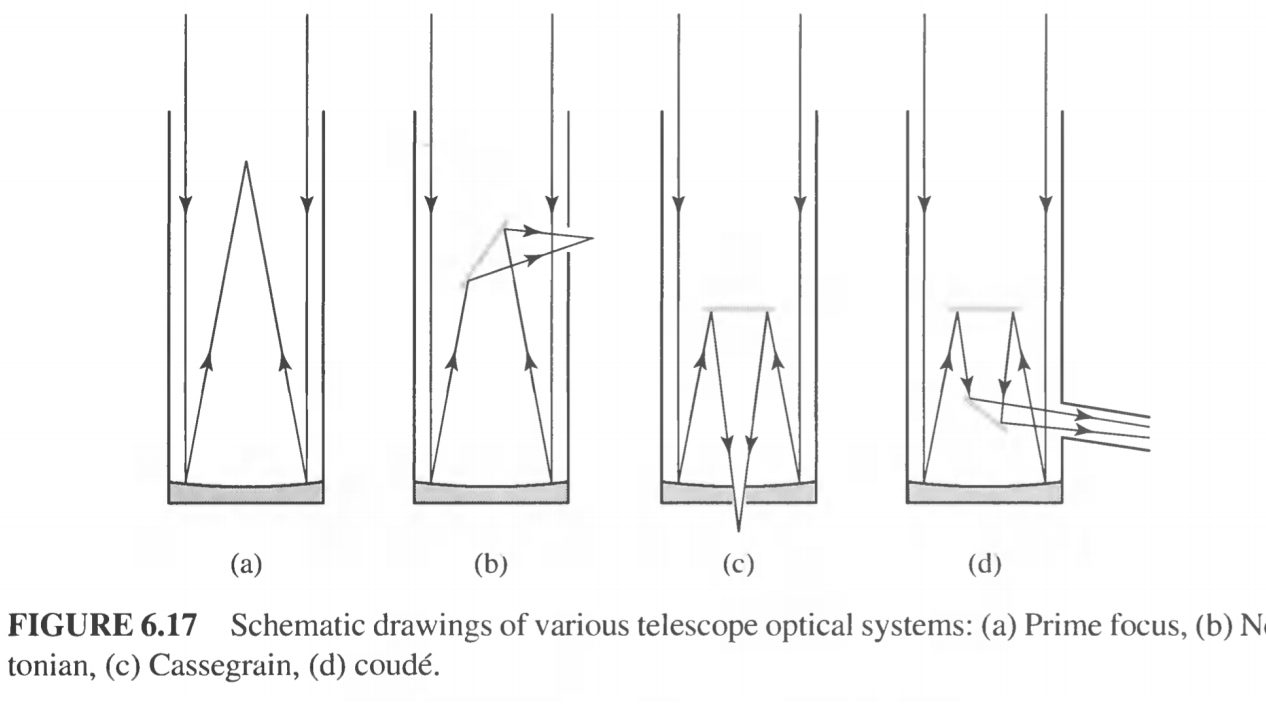
\includegraphics[scale=0.5]{Figures/Telescopes.png}
\begin{enumerate}[label=(\alph*)]
 \item \textbf{Prime focus:} Placing a detector can actually block some of the light, which is a drawback
 \item \textbf{Newtonian:} Solves that problem, but the detector needs to be placed far away from the center of mass, which can lead to a huge gravitational torque
 \item \textbf{Cassegrain:} Solves the previous problem, instrument package and detector can be placed at bottom
 \item \textbf{Coude:} Light can be reflected to a laboratory where more complex analysis can be conducted
 \item \textbf{Schmidt:} Provides a wide field of view
\end{enumerate}

\textbf{Charge-Coupled Device:} A photon detector which acheives a very high efficiency (detects almost all photons) by counting the electrons in excited states after struck by photons (which give them energy)

\subsection{Radio Telescopes}
$$P = \int\int S(\nu)f_{\nu}d\nu dA$$, where $S(\nu)$ is the spectral flux density

One benefit of radio astronomy is that dishes do not need to be as precise for longer wavelengths. Additionally, multiple dishes can be used to measure the location of a source. Note that based on the standard interference conditions, $$\sin\theta = \frac{L}{d}$$ The larger the distance between them, the greater the angular resolution (examples include radio dish arrays set across different continents and the VLA in Mexico)\newline
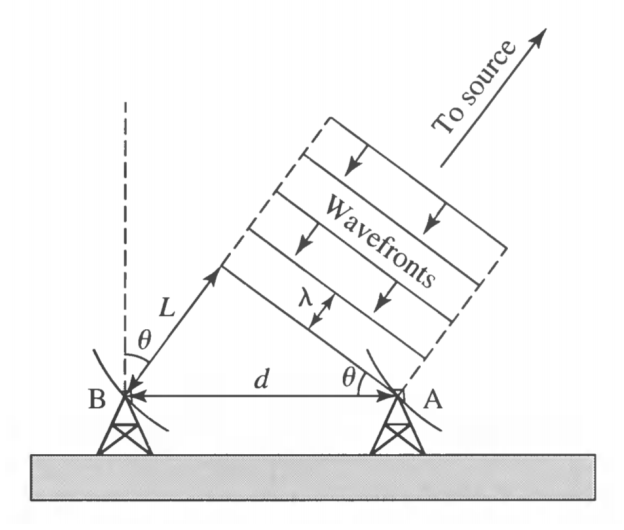
\includegraphics[scale=0.5]{Figures/VLA.png}
\subsection{Astronomy in Different Wavelength Regions}

Transparency of the atmosphere is one issue when considering observational astronomy in different wavelengths:\newline
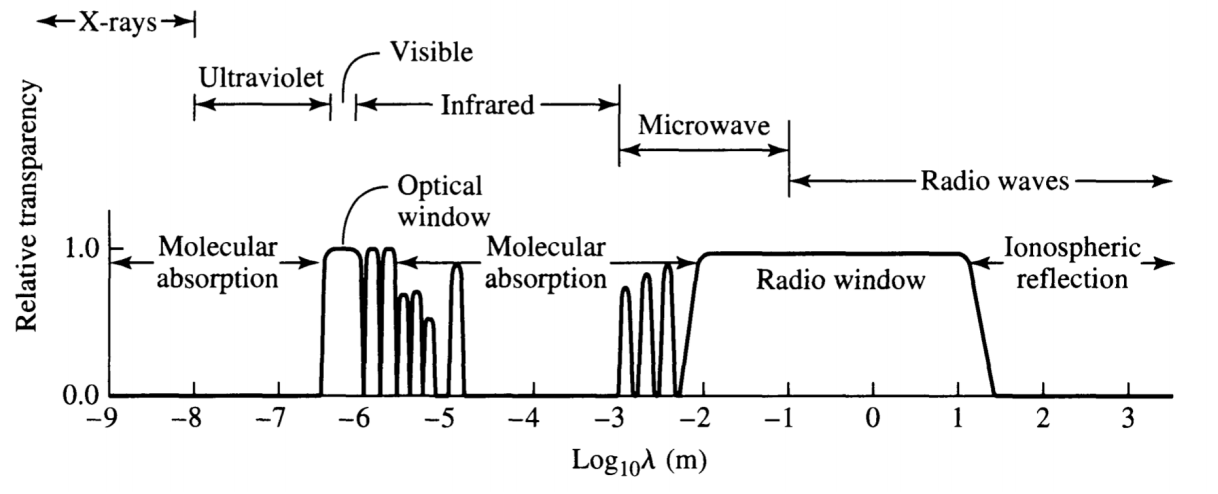
\includegraphics[scale=0.5]{Figures/WavelengthTransparency.png}

Short-wavelength astronomy can yield info about high energy objects like neutron stars and black holes. Methods like Bragg scattering in crystals must be used to observe high frequency wavelengths like x-ray, UV, and gamma because:
\begin{itemize}
    \item Small wavelengths $\implies$ less room for imperfections in lens design
    \item Glass can be opaque to short-wavelength photons, and on the other hand, high energy photons may pass right through reflecting surfaces
\end{itemize}

\section{Binaries}
\begin{itemize}
    \item \textbf{Optical Double:} Not actually a binary system, two stars that are on the same line of sight
    \item \textbf{Visual Binaries:} Both stars can be easily resolved
    \begin{itemize}
        \item $m_1r_1 = m_2r_2$ (used to determine mass ratios based on distance from COM)
        \item $a = d\alpha$, and a factor of $\cos{i}$ can be used to factor in inclination angle 
    \end{itemize}
    \item \textbf{Astrometric Binary:} Only one member can be observed, but an abnormal radial velocity curve leads us to infer the presence of another object (which is usually smaller)
    \begin{itemize}
        \item If only one star visible, the following \textbf{mass function} can be determined:
        $$\frac{m_2^3}{(m_1 + m_2)^2}\sin^3{i} = \frac{P}{2\pi G}v_{1r}^3$$
        \item This is one of the main ways that we look for planets and stars (their gravitational effects on other visible stars)
    \end{itemize}
    \item \textbf{Eclipsing Binary:} If orbital planes are along line of sight, one star may temporarily and periodically eclipse the other (minima present in light curves)
    \begin{itemize}
        \item Inclination angle $i$ must be relatively close to $90^{\circ}$ (actually, the average value of $\sin^3 i$ is around $2/3$ due to this selection effect)\newline
        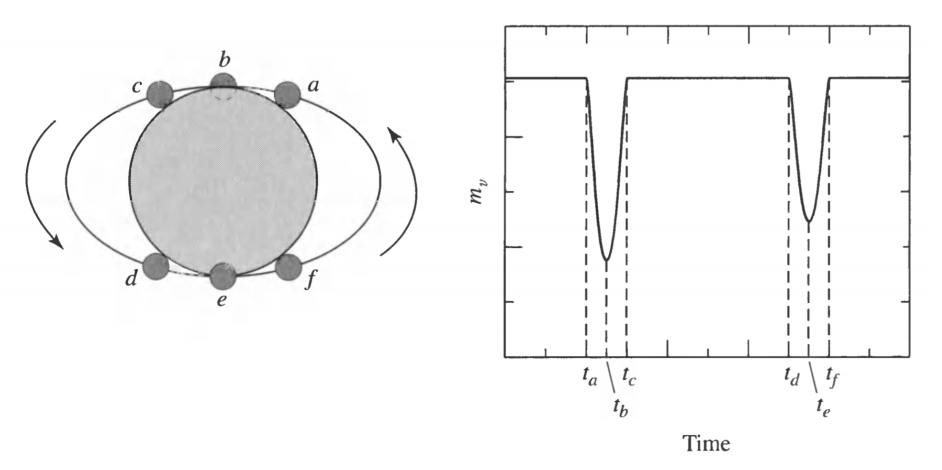
\includegraphics[scale=0.7]{Figures/EclipsingBinaries.png}
        \item Radius and temperature can be determined to some extent from light curve data
        $$r_s = \frac{v_{\text{rel}}}{2}(t_b - t_a)$$ $$r_l = \frac{v_{\text{rel}}}{2}(t_c - t_a) = r_s + \frac{v_{\text{rel}}}{2}(t_c - t_b)$$
        Additionally, $$\frac{B_0 - B_P}{B_0 - B_S} = \frac{F_s}{F_l} = \left(\frac{T_s}{T_l}\right)^4$$
    \end{itemize}
    \item \textbf{Spectrum Binary:} Stars' velocities can be determined based on their red/blueshift and the Doppler effect. When one of the spectra is blueshifted, the other one would be redshifted (since stars are traveling in opposite directions); the spectra allow them to be indentified.
\end{itemize}

Computer modeling can also play an important role in determing characteristics of the members of binary systems.

\section{Stellar Atmospheres}

\subsection{Describing/Quantifying Radiation}

\textbf{Specific intensity:} $I_{\lambda} = \dv{I}{\lambda} = \frac{E_{\lambda}\;\dd \lambda}{\dd \lambda\;\dd t\;\dd A\cos\theta\;\dd \Omega}$

Mean intensity can be found by integration, for blackbody radiation $\left<I_{\lambda}\right> = B_{\lambda}$

\textbf{Specific energy density:} $u = \frac{4\pi}{c}\int_{0}^{\infty}B_{\lambda}(T)\;\dd \lambda = \frac{4\sigma T^4}{c} = aT^4$ ($a$ is defined as \textit{radiation constant}).

"Photon gas" also produces \textbf{radiation pressure} $\implies$ for blackbody radiation, $P_{\text{rad}} = \frac{4\pi}{3c}\int_{0}^{\infty}B_{\lambda}\;\dd \lambda = \frac{4\sigma}{3c}T^4 = \frac{1}{3}aT^4 = \frac{1}{3}u$.

\subsection{Temperature}

Absorption lines due to stellar opacity $\implies$ \textbf{line blanketing} occurs, meaning that spectrum changes and differs from ideal blackbody $\implies$ \textit{difficult to determine "effective" temperature}.

\textbf{Types of Temperature}:
\begin{itemize}
    \item \textbf{Effective Temperature:} Based on Stefan-Boltzmann Law (luminosity)
    \item \textbf{Excitation Temperature:} Based on Boltzmann equation (ratio of particles in diff energy levels)
    \item \textbf{Ionization Temperature:} Based on Saha equation (ratio of ioniziation levels)
    \item \textbf{Kinetic Temperature:} Based on Maxwell-Boltzmann distribution
    \item \textbf{Color Temperature:} Based on fitting curve to Planck curve
\end{itemize}

If temperature gradient is very gradual compared to movement of particles (e.g. mean free path) $\implies$ \textbf{local thermal equilibrium (LTE)} (temp. approx. constant)

\textbf{Mean free path:} $\ell = \frac{1}{n\sigma}$, where $n$ is number density and $\sigma$ is cross section (e.g. $2a_0$ for H)

\subsection{Stellar Opacity}

Definition of \textbf{opacity or absorption coeff.} $\kappa_\lambda$ based on change in intensity: $dI_\lambda = -\kappa_\lambda\rho I_\lambda\;\dd s$ $\implies$ exponential decay of intensity

Definition of \textbf{optical depth:} $\dd \tau_\lambda = -\kappa_\lambda\rho\;\dd s$ (so that $dI_\lambda = -\tau_\lambda I_\lambda$)
\begin{itemize}
    \item Number of mean free paths along ray's path
    \item Maximum seeing limit about $\tau_\lambda \approx 1$
    \item \textit{Optically thin:} $\tau_\lambda \ll 1$, \textit{optically thick:} $\tau_\lambda \gg 1$ (defined on a wavelength basis)
\end{itemize}

\subsubsection{Sources of Opacity}
Absoprtion/scattering change path of photons, contribute to opacity. Total opacity is sum of contributions from each of factors mentioned below.
\begin{itemize}
    \item \textbf{Bound-bound transitions:} electron changes orbitals, absorbs and releases photons; $\kappa_{bb}$ relatively low except at certain wavelengths due to quantization of energy in photons that can be absorbed $\implies$ sharp changes lead to absorption lines
    \item \textbf{Bound-free absorption:} photon ionizes atom, no quantization of energy restriction (only requirement is $\lambda \leq hc/E_\text{ionization}$) $\implies$ source of continuum opacity. Also leads to \textbf{Balmer jump}, or sudden increase in opacity when $\lambda \leq hc/E_\text{ionization}$
    \item \textbf{Free-free absorption:} Free electron close to ion can absorb photon (increasing speed) $\implies$ continuum opacity; electron can also emit photon (slows down) - \textit{bremsstrahlung}, or "braking radiation"
    \item \textbf{Electron scattering:} Photons scattered by electrons (Thomson scattering, Compton scattering, or Rayleigh scattering) $\implies$ continuum opacity, prevalent at high temps where most electrons are free (atoms are ionized)
    \item \textbf{H\textsuperscript{-} ion:} For late type stars (i.e. after F0), H\textsuperscript{-} ions contribute to continuum opacity because they can be easily photoionized by a wide range of photon wavelengths (low binding energy)
\end{itemize}

\textbf{Roseland Mean Opacity:} $\dfrac{1}{\overline{\kappa}} = \dfrac{\int_{0}^{\infty}\frac{1}{\kappa_\nu}\pdv{B_\nu}{T}}{\int_{0}^{\infty}\pdv{B_\nu}{T}}$
\begin{itemize}
    \item Increases w/ density, decreases w/ temperature
\end{itemize}

\subsection{Radiative Transfer}
Absorption and emissions processes balance each other to form an equilibrium, as photons are scattered, redirected, emitted, and absorbed $\implies$ photons move along a \textbf{random walk}. $$d = \ell\sqrt{N} = \tau_\lambda\ell \implies N = \tau_\lambda^2$$

Thus, photons need to be about $\tau_\lambda < 1$ away from the surface in order to be able to escape $\implies$ we can only see about $\tau_\lambda \approx 2/3$ into stellar atmospheres (average point of origination of photons).
\begin{itemize}
    \item \textbf{Limb darkening:} Since our line of sight is not straight into the star when viewing top and bottom, same optical depth does not allow us to see as deeply into it $\implies$ "limbs" seem to be darker
    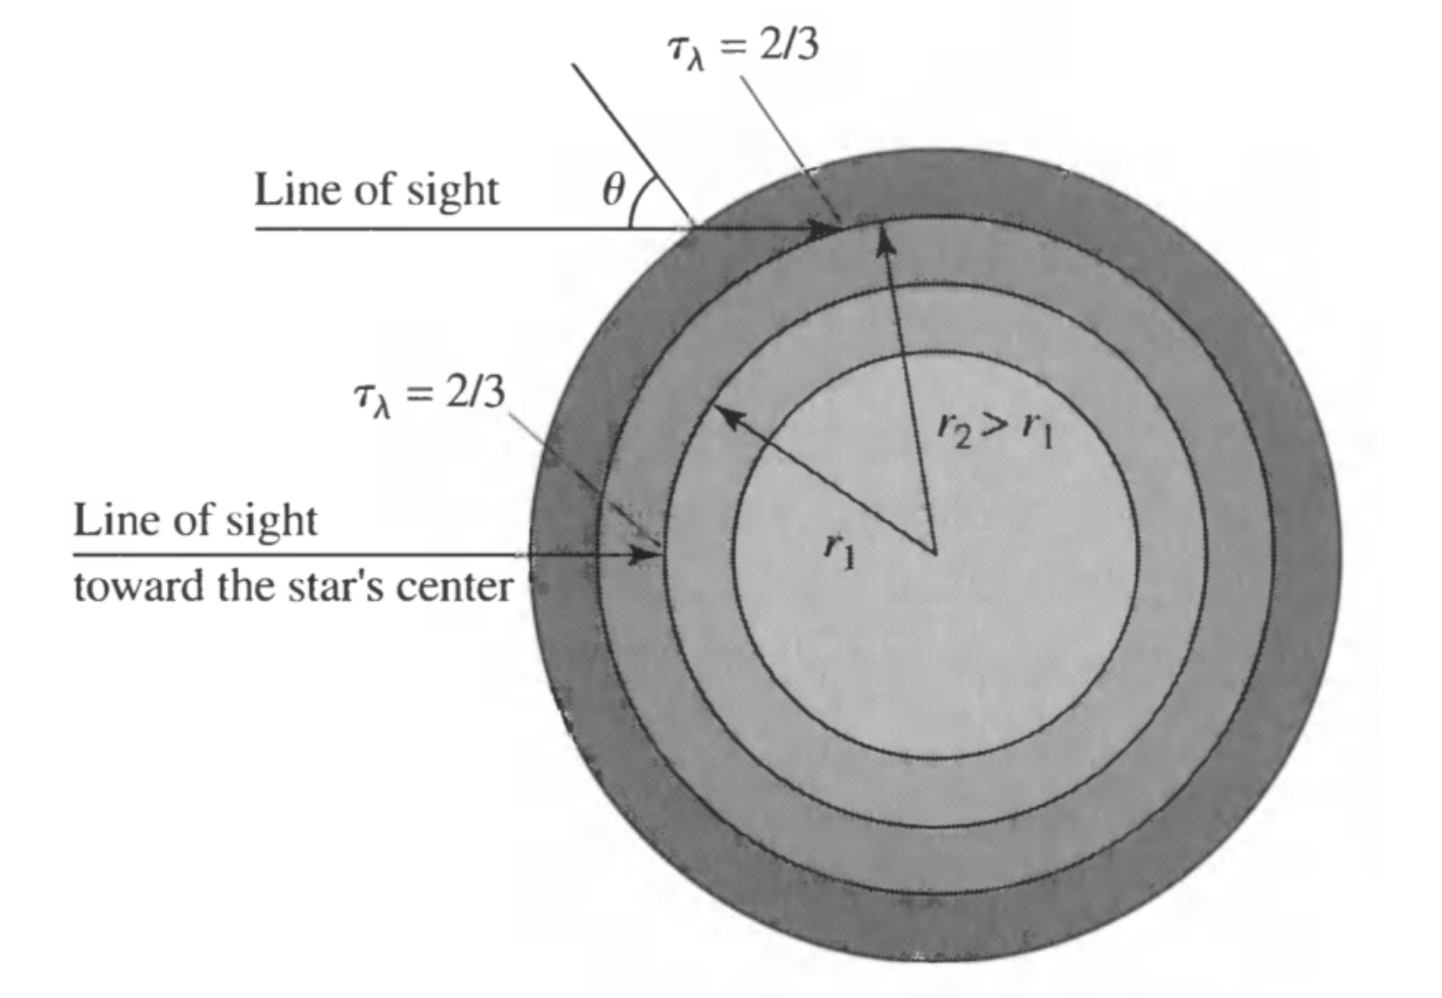
\includegraphics[scale=0.5]{Figures/LimbDarkening.png}
 \end{itemize}

\subsubsection{Transfer Equation}

Accounting for both emission and absorption, $\dd I_\lambda = -\kappa_\lambda\rho I_\lambda\;\dd s + j_\lambda\rho\;\dd s$, where $j_\lambda$ is the \textbf{emission coefficient} for certain wavelength. Then, $$\boxed{-\dfrac{1}{\kappa_\lambda\rho}\dv{I_\lambda}{s} = \dv{I_\lambda}{\tau_\lambda} = I_\lambda - S_\lambda}$$ where $S_\lambda \equiv j_\lambda/\kappa_\lambda$ is the \textbf{source function}.

Then, if LTE is assumed, $\dv{I_\lambda}{s} = 0 \implies S_\lambda = B_\lambda$ (so that $I_\lambda - S_\lambda = 0$ in transfer eq.)

Integrating the transfer equation over all angles and simplifying, $$\boxed{\dv{P_\text{rad}}{\tau_\nu} = \frac{1}{c}F_\text{rad}}$$ Qualitatively, the equation shows that pressure gradient $\implies$ radiative flux.


\section{Interior of Stars}

\textbf{Hydrostatic Equilibrium condition:} $\dv{P}{r} = -\rho g$
\textbf{Mass Conservation equation:} $\dv{M_r}{r} = 4\pi r^2\rho$
\textbf{Luminosity Gradient equation:} $\dv{L_r}{r} = 4\pi r^2\rho\epsilon$, where $\epsilon \equiv \frac{dL}{dm}$

\subsection{Stellar Energy Sources (e.g. Nuclear):}
Total mechanical energy can be found to be $$E \sim -\frac{3}{10}\frac{GM^2}{R}$$ by integrating over shells and assuming density is constant (along with applying Virial theorem) $\implies$ total lifetime would be $t_{KH} \sim E/L$ (\textbf{Kevin-Hemholtz timescale})
\begin{itemize}
    \item Too short of an estimate (only around 10\textsuperscript{7} yr. for the sun) $\implies$ \textbf{mechanical energy cannot be only source of energy}
\end{itemize}

\textbf{Nuclear energy} (fission and fusion reactions, binding energy) accounts for most of star's energy.
\begin{itemize}
    \item Although temperature not high enough for atoms to overcome Coloumb barrier clasically, Heisenberg uncertainty principle leads allows \textbf{quantum tunneling}, since uncertainty in position makes it possible for atoms to get close enough to each other to have a nuclear reaction.
    \item The probability of reaction depends on the energy of collision; the \textbf{Gamow peak} is a result of the tradeoff between easier Coloumb barrier penetration and the exponentially decaying Maxwell-Boltzmann distribution at higher energy levels.\newline
    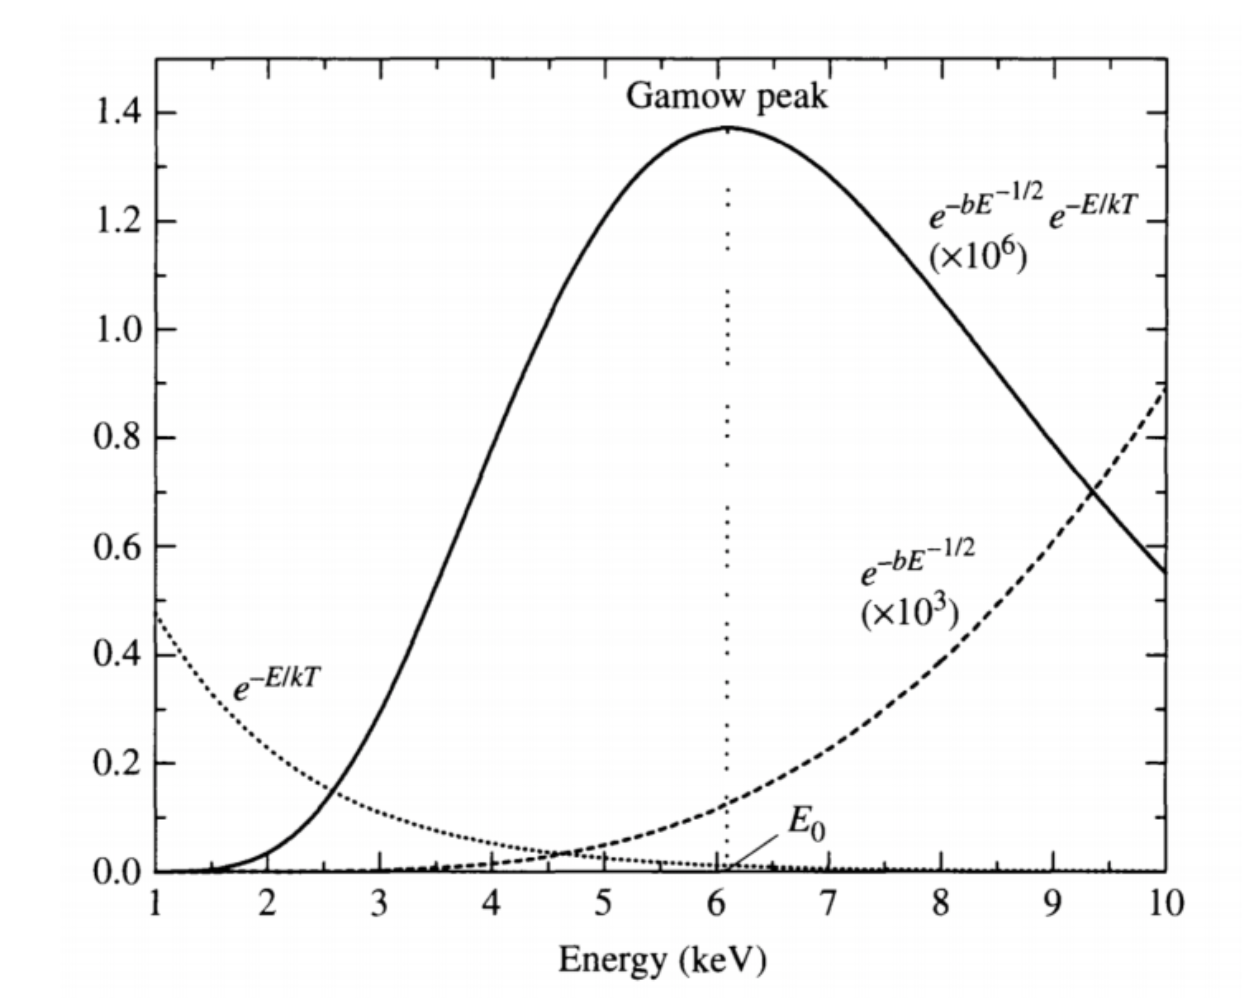
\includegraphics[scale=0.6]{Figures/GamowPeak.png}
\end{itemize}

\subsubsection{Types of Nuclear Reactions}
\begin{itemize}
    \item \textbf{PP Chain Reaction}\newline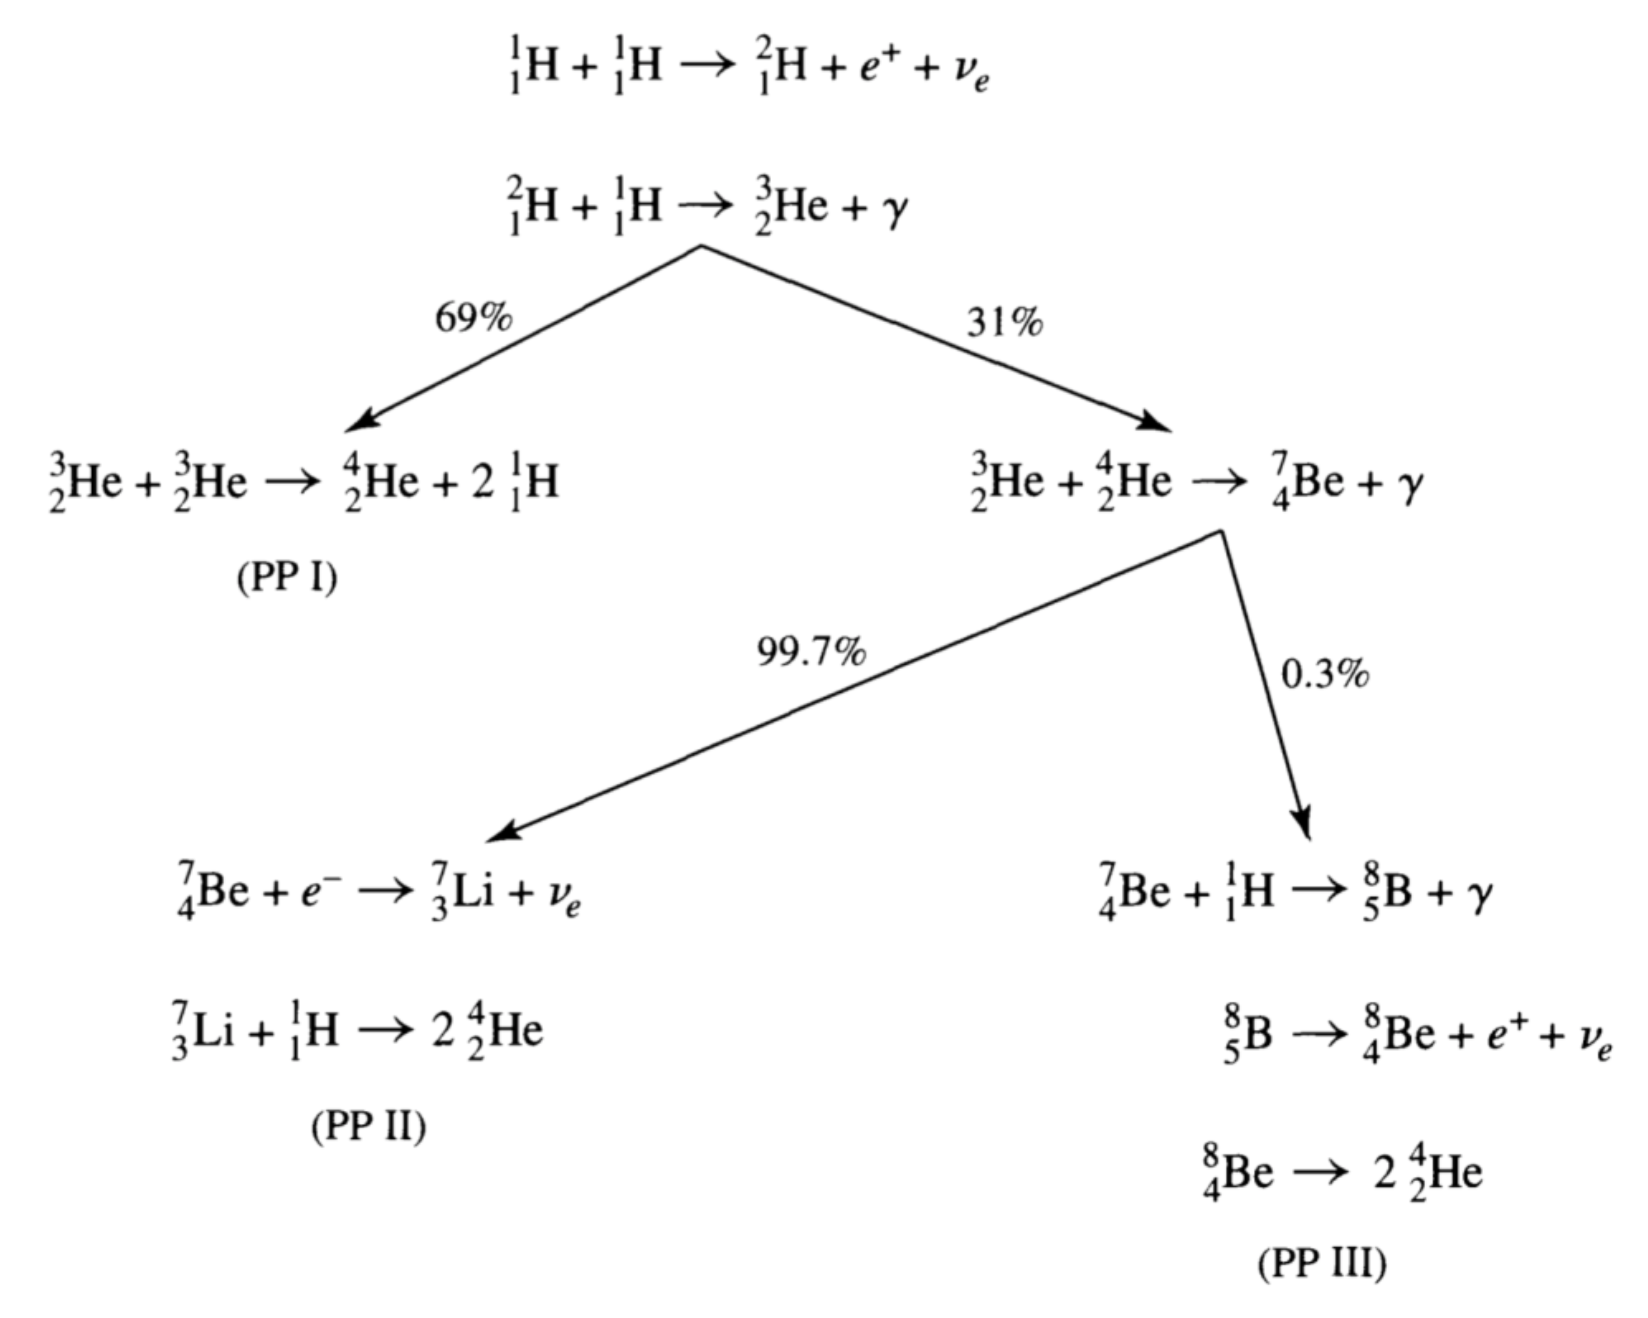
\includegraphics[scale=0.4]{Figures/PPChain.png}
    \item \textbf{CNO Cyle:} Dominates at higher temperatures due to extremely high temperature dependence \newline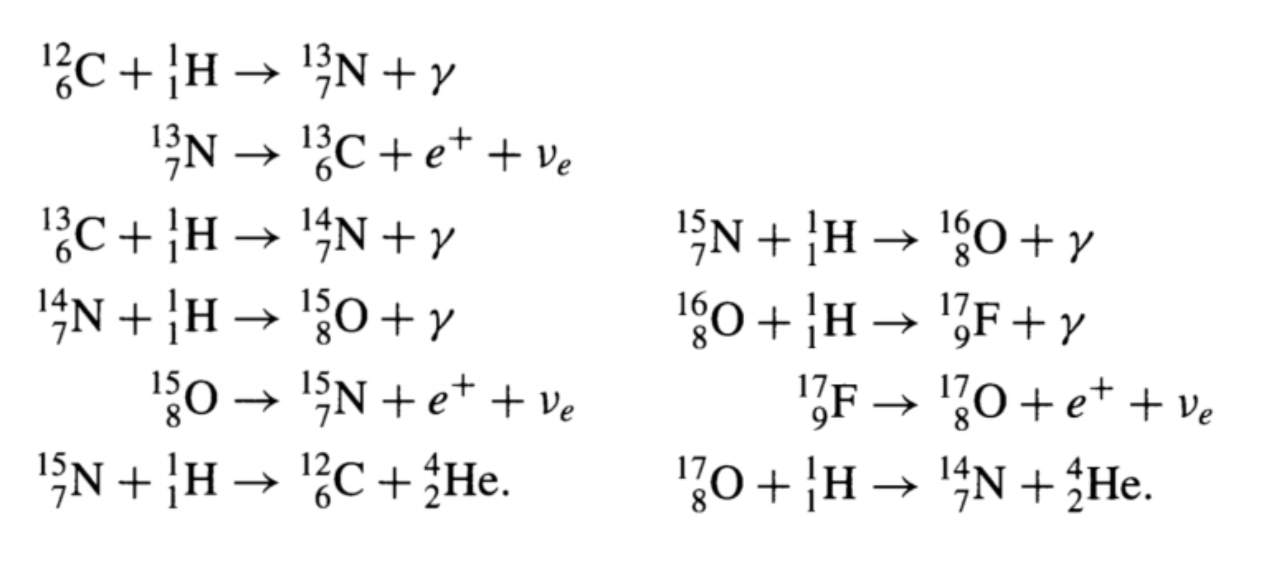
\includegraphics[scale=0.4]{Figures/CNO.png} 
    \item \textbf{Triple Alpha Reaction:} Unstable Be nucleus needs to be struck almost immediately (this reaction is even more temperature dependent than CNO)\newline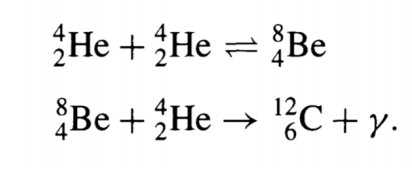
\includegraphics[scale=0.5]{Figures/TripleAlpha.png}
    \item \textbf{Carbon and Oxygen Burning:} Carbon and oxygen atoms (after they become abundant) can capture alpha particles or react with themselves to burn (reactions with *** are endothermic, relatively rare)\newline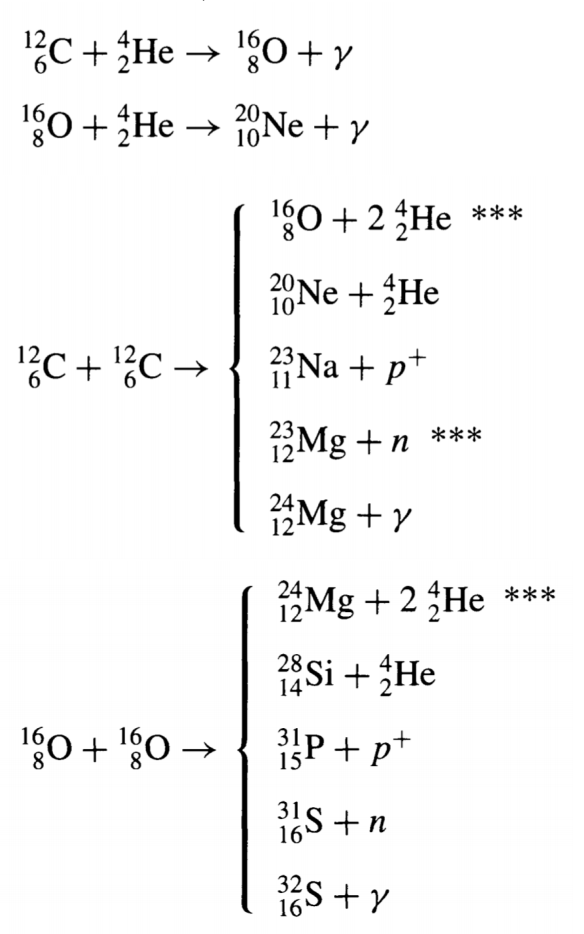
\includegraphics[scale=0.7]{Figures/COBurning.png}
\end{itemize}

Below is a \textbf{binding energy} curve ($E_b = \Delta mc^2$ from relativity). Iron (Fe) is most stable $\implies$ final element that fusion can produce.\newline
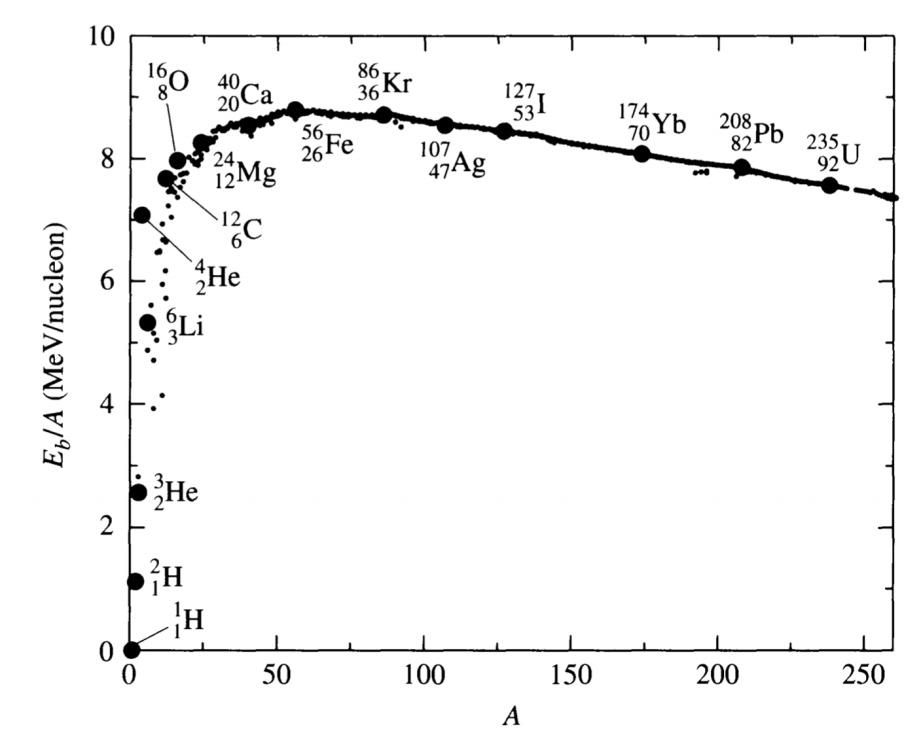
\includegraphics[scale=0.5]{Figures/BindingEnergyCurve.png} 

\textbf{Types of Energy Transport Mechanisms:}
\begin{itemize}
    \item \textbf{Radiation:} Photons can carry energy to the surface
    \item \textbf{Convection:} Hot, low-density matter can rise and carry energy to the surface as a result of its buoyancy
    \item \textbf{Conduction:} Collisions between particles lead to energy transfer.
\end{itemize}

\textbf{Radiative Pressure Gradient:} Since we know that $P_{\text{rad}} = \frac{1}{3}aT^4$ and $F_{\text{rad}} = L_r/4\pi r^2$, we can substitute into $\dv{P_{\text{rad}}}{r} = -\frac{\kappa\rho}{c}F_\text{rad}$ to get: $$\boxed{\dv{T}{r} = -\frac{3}{4ac}\frac{\kappa\rho}{T^3}\frac{L_r}{4\pi r^2}}$$

\textbf{Pressure Scale Height:} Characteristic length scale for convection: $$\frac{1}{H_P} \equiv -\frac{1}{P}\dv{P}{r} \implies \boxed{H_P = \frac{P}{\rho g}}$$

\textbf{Adiabatic Temperature Gradient:} Noting that $P = K\rho^\gamma$, it can be shown that $$\dv{T}{r} = -\left(1 - \dfrac{1}{\gamma}\right)\frac{\mu m_H}{k}\frac{GM_r}{r^2} = -\dfrac{g}{C_P}$$
\begin{itemize}
    \item The condition for convection can be shown to be $\dfrac{\d(\ln P)}{\d(\ln T)} < \dfrac{\gamma}{\gamma - 1}$
\end{itemize}

Keeping in mind the \textbf{Vogt-Russell Theorem} (a star's mass and composition uniquely determine its entire internal structure and evolution), stellar models can be constructed numerically (too complicated to be done analytically).

\section{Interstellar Medium}
\textbf{Gas and dust between the stars}
\subsubsection{Interstellar Extinction}
ISM can block light, leading to a lower apparent magnitude;
\begin{itemize}
    \item Magnitudes of extinction $A_\lambda = 2.5\tau_\lambda \log_{10}e$
    \item High wavelengths unaffected, short wavelengths blocked (unless they miss the dust) $\implies$ leads to \textbf{interstellar reddening} and blue \textbf{reflection nebula} opposite to cloud direction
    \item Materials like graphite, silicates, and complex organic molecules
\end{itemize}
\subsubsection{Hydrogen}
ISM is ~70\% Hydrogen (H2, H I/II). 
H I is hard to detect (no emission lines, absorption only in UV. However, can be rarely be identified through \textbf{21-cm line} (direction of spin flip leads to change in energy). Usually present around molecular dust clouds (protected from UV radiation, etc.)\newline
\textbf{Tracer molecules} such as CO, CH, OH, etc. are used to approximate H2 levels (hard to measure directly).

Heated by cosmic rays, cooled by IR photons.

\subsubsection{Types of Interstellar Clouds:}
Diffuse/translucent molecular clouds, dark cloud complexes, clumps, dense cores, hot cores, Bok globules, etc.

\subsection{Formation of Protostars}
Using the Virial theorem ($2K + U$) and substituting expressions for KE, GPE, and solving, we get that the minimum mass and radius (\textbf{Jean's mass/radius}) for a protostar to form are:
\begin{align*}
M_J \approx \left(\frac{5kT}{G\mu m_H}\right)^{3/2}\left(\frac{3}{4\pi\rho_0}\right)^{1/2} \\
R_J \approx \left(\frac{15kT}{4\pi G\mu m_H\rho_0}\right)^{1/2}
\end{align*}
\textbf{Bonnor-Ebert mass} takes into account pressure of ISM: 
\begin{align*}
M_{\text{BE}} = \dfrac{1.18(kT/\mu m_H)^2}{\sqrt{P_0G^3}}
\end{align*}
\textbf{Homologous Collapse:} When density is relatively uniform, all parts of the cloud collapse in the same time of free-fall: 
\begin{align*}
t_{ff} = \left(\dfrac{3\pi}{32}\dfrac{1}{G\rho_0}\right)^{1/2}
\end{align*} 
\textbf{Inside-out collapse} occurs when density is nonuniform, inside collapses faster.
\begin{itemize}
\item However, magnetic field can resist collapse which can lead to collapse not really being free-fall $\implies$ greater time of collapse (lining up with observations)
\end{itemize}
Large molecular clouds don't collapse into one large star, but rather \textbf{fragmentation} occurs (different parts of the cloud themselves collapse into smaller stars when they surpass the Jean's mass/radius).
\begin{itemize}
    \item Increase in temperature increases Jean mass's $\implies$ fragmentation stops at some point
\end{itemize}

Other factors like turbulence, magnetic fields, etc. are involved too, made clear by disparity in calculated and actual time of collapse.
\begin{itemize}
    \item Magnetic fields resist collapse, increasing collapse time $\implies$ if a star has too low of a mass (\textbf{magnetically subcritical}), will not collapse, and vice versa (\textbf{supercritical})
    \item \textbf{Ambipolar diffusion}, movement of neutral particles, may also contribute to collapse
\end{itemize}

Collapse is initially isothermal, but as star gets denser and denser, light is blocked, making it more adiabatic. Supersonic speeds of material falling cause shockwaves, and lead to huge increases in temperature, until deteurium eventually runs out.

\subsection{Pre-Main Sequence Evolution}
Much slower than formation of protostar, on Kevin-Hemholtz timescale.

\textbf{Hayashi Track}:
Contribution of H- ions to opacity leads to huge convective zone $\implies$ vertical line on HR diagram, right of which stable stars can't exist (too low temp)

\section{Cosmology}
\textbf{Olber's Paradox:} If there are infinitely many stars, why is the sky dark? $\implies$ Because light takes time to travel so we only see a finite part of the universe.

\textbf{Cosmological Principle:} Universe is homogeneous and isotropic.

\textbf{Scale factor and redshift}:
\begin{align*}
    R(t) = \frac{1}{1 + z} \\
    \rho(z) = \rho_0(1 + z)^3
\end{align*}

\textbf{Critical density} for a flat universe:
\begin{align*}
    \rho_c(t) = \frac{3H(t)^2}{8\pi G}
\end{align*}
\textbf{Density parameter definition}:
\begin{align*}
    \Omega(t) = \frac{8\pi G\rho(t)}{3H^2(t)}
\end{align*}
For baryonic matter $\Omega_{b, 0} \approx 0.04$, for dark and baryonic matter $\Omega_{m, 0} \approx 0.27$.

\begin{itemize}
    \item $\Omega_0 > 1$, universe is closed (will eventually collapse)
    \item $\Omega_0 = 1$, universe is flat (will expand but at a slowing rate)
    \item $\Omega_0 < 1$, universe will continue to expand rapidly
\end{itemize}
Behavior remains consistent throughout the cycle of the universe, our universe seems to be \textbf{flat}.

\textbf{Lookback Time}: $t_L = t_0 - t(z)$ (How far in the past is an object with redshit $z$)

\textbf{Fluid Equation}: $\dv{(R^3\rho)}{t} = -\frac{P}{c^2}\dv{(R^3)}{t}$
Pressure in the universe serves to slow down the expansion, $$\frac{\partial^2R}{\partial t^2} = -\frac{4}{3}\pi G(\rho + 3P/c^2)R$$
\begin{itemize}
\item Illustrates \textbf{Birkhoff's theorem}, which says Einstein's field eq. only have one sol for spherically symmetric mass distribution
\end{itemize}
\textbf{Deacceleration Parameter}: $$-\frac{R(t) d^2R/dt^2 }{(dR/dt)^2}$$

\subsection{CMB}

Age of universe could not be $t = 1/H$, this was shorter than Earth's age
\end{document}

